\documentclass[10pt,journal,letterpaper]{IEEEtran}
\usepackage[letterpaper, left=0.65in, right=0.65in, bottom=0.7in, top=0.7in]{geometry}
\usepackage{tikz}
\usetikzlibrary{arrows.meta}
\usepackage{mathptmx}
\usepackage{lipsum}
\usepackage{cite}
\usepackage{amsmath,amssymb,amsfonts}
\usepackage{algorithmic}
\usepackage{graphicx}
\usepackage{textcomp}
\usepackage{xcolor}
\usepackage{nicefrac}
\usepackage{type1cm}
\usepackage{lettrine}
\usepackage{makecell}
\usepackage{fancyhdr}
\usepackage[none]{hyphenat}
\usepackage{float}
\usepackage{hyperref}
\usepackage{multirow}
\usepackage{import}
\usepackage{xifthen}
\usepackage{pdfpages}
\usepackage[siunitx]{circuitikz}
\usepackage{siunitx}
\usepackage{transparent}
\usepackage{microtype}

\graphicspath{ {./figures/} }

\newcommand{\incfig}[1]{%
	\centering
    \import{./figures/}{#1.pdf_tex}
}
    
\pagestyle{fancy}
\fancyhf{}
\renewcommand{\headrulewidth}{0pt}
\rhead{\thepage}
\lhead{Lab Final}

\setlength{\columnsep}{0.2in}
\setlength{\columnwidth}{3.5in}

\sisetup{per-mode = symbol,
	inter-unit-product = \ensuremath{{}\cdot{}}
}

\begin{document}
\title{Title Here}

\author{\IEEEauthorblockN{\huge{Hornilla, Joshua \\ Hutt, Kateland \\ Latzko, Alexander \\ Sukhadia, Kenni \\}}
\IEEEauthorblockA{
Group 50 \quad April 22, 2022}
}

\maketitle
\thispagestyle{empty}

\newcommand{\todo}{\textcolor{red}{???}}

\begin{abstract}
This experiment uses knowledge of the two-dimensional principal stress state to determine the internal pressure in an unopened soda can.
Thin-walled pressure vessel theory is used in conjunction with theories on principal stresses to report the internal can pressure.
This result is compared to another method based upon the ideal gas law.
The hoop stress in the can is 78.11 $\pm$ 1.128 MPa and the longitudinal stress is 46.27 $\pm$ 0.677 MPa.
The internal pressure reported by the mechanics of materials approach is 252 $\pm$ 43.40 kPa.
The internal pressure reported by the ideal gas law method is 258 $\pm$ 57.15 kPa.
\end{abstract}

\begin{IEEEkeywords}
plane stress, principal stresses, strain gauge rosette, thin-walled pressure vessel
\end{IEEEkeywords}

\section{Introduction}
\IEEEPARstart{C}{ylindrical} pressure vessels are an effective way to store gasses or liquids which must be kept at certain high pressures.
As such, knowing the operating and current pressures in these vessels is imperative to ensuring user safety; catastrophic failures in these vessels can sometimes be fatal.
The stresses in the walls of these vessels can be used to determine the overall pressure within the vessel.
This study seeks the pressure in a sealed soda can.

The can is a thin-walled pressure vessel.
The diameter of the can is much greater than its wall thickness, leading to the assumption that there is no stress in the direction of the thickness of the can, so the stresses in the vessel wall can be analyzed as a two-dimensional stress state, the plane stress condition.

To analyze this stress state, strain gauges can be affixed in a 0-45-90$^\circ$ rosette on the side of the can to record the strains on the walls.
Using multiple strain gauges allows an experimenter to determine the complete strain state, including the shear strain.
As the strain gauge is a transducer, the strains are recorded as a voltage difference, $\Delta V_{g}$, and are calculated according to \eqref{eq:strain}, where $V_s$ is the excitation voltage for the circuit, $G_f$ is the gauge factor of the strain gauge, given by the manufacturer, and $A$ is the gain of the amplifier.
\begin{equation}
\label{eq:strain}
\varepsilon=\frac{4\Delta V_g}{A V_s G_f}
\end{equation}

These strain gauges work in conjunction with a quarter Wheatstone bridge circuit to record meaningful voltage differences (Fig. \ref{fig:Wheat}).
The strain gauge acts as a variable resistor.
The change in voltage across the bridge as the strain gauge moves and varies its resistance is the voltage used to compute strain in \eqref{eq:strain}.
Each member of the strain gauge rosette has its own individual Wheatstone bridge circuit fed by an excitation voltage.

\begin{figure}[H]
\centering
\begin{circuitikz}[american voltages, scale=2]
\ctikzset{label/align = straight}
  \draw (0,0) to[V, invert, l_=$V_s$] (0,2) -- (2,2)
  to[R, l_=$R_4$,*-*] (1,1)
  to[R, l_=$R_3$, *-*] (2,0) -- (0,0);

 \draw (2,2) to[R=$R_1$, *-*] (3,1) to (2.9,0.9) to (3.3,0.9) to[european resistor=$R_2$] (3.3,0.1) to (2.1,0.1) to (2,0);
 \draw (1,1) to[rmeter, t=$V_g$] (3,1);
 \draw (3.3,0.5) node[left=0.8em,align=left] {Strain\\gauge};
 \end{circuitikz}
\label{fig:Wheat}
\caption{A simple quarter Wheatstone bridge circuit.}
\end{figure}

In plane strain, the shear strain $\gamma_{xy}$ can be computed using the 45$^\circ$ strain gauge value according to \eqref{eq:strainThet}, where $\varepsilon_x$ and $\varepsilon_y$ are the strains from the 0$^\circ$ and 90$^\circ$ strain gauges, and $\theta$ is 45$^\circ$ for this rosette \cite{b5}.
\begin{equation}
\label{eq:strainThet}
\varepsilon_\theta=\frac{\varepsilon_x+\varepsilon_y}{2}-\frac{\varepsilon_x-\varepsilon_y}{2}\cos(2\theta)+\gamma_{xy}\sin(2\theta)
\end{equation}

While the experimenter should attempt to align the strain gauge rosette along the principal axes, along the can's central axis and along its circumference, the true principal strain should be found according to \eqref{eq:princStrain}, where $\varepsilon_{1,2}$ are the principal strains for the plane strain condition.
This is based upon the concepts of Mohr’s circle, a geometric way to identify principal stresses and strains in a material.
\begin{equation}
\label{eq:princStrain}
\varepsilon_{1,2}=\frac{\varepsilon_x+\varepsilon_y}{2} \pm \sqrt{\left(\frac{\varepsilon_x-\varepsilon_y}{2}\right)^2+\left(\frac{\gamma_{xy}}{2}\right)^2}
\end{equation}

With principal strains in hand, the principal stresses in the vessel can thus be computed.
These principal stresses in the wall arise from the internal pressure pushing on the can wall, so knowing the principal stresses in the wall may lead to the pressure within the can.
In 2D strain, the well-known Hooke’s law relating stress to strain is given directionally as \eqref{eq:sigma1} and \eqref{eq:sigma2}, where $\sigma_{1,2}$ are the principal stress on the wall, $E$ is the modulus of elasticity for the can material, aluminum alloy, $\nu$ is Poisson’s ratio, and $\varepsilon_{1,2}$ are the principal strains, found by using \eqref{eq:princStrain} with the recorded strains \cite{b1}.
\begin{subequations}
\label{eq:sigmas}
\begin{align}
\sigma_1&=\frac{E}{1-\nu^2}\left(\varepsilon_1+\nu\varepsilon_2\right) \label{eq:sigma1} \\
\sigma_2&=\frac{E}{1-\nu^2}\left(\varepsilon_2+\nu\varepsilon_1\right) \label{eq:sigma2}
\end{align}
\end{subequations}
For thin-walled pressure vessels, the 2D stress state is described by the longitudinal stress, along the vessel's central axis, and hoop stress, along its circumference, which can be computed with the principal strains above.
The free-body diagram (Fig. \ref{fig:PVessel}) can be a helpful tool in relating these stresses to the can's internal pressure \cite{b1}.

\begin{figure}[H]
\centering
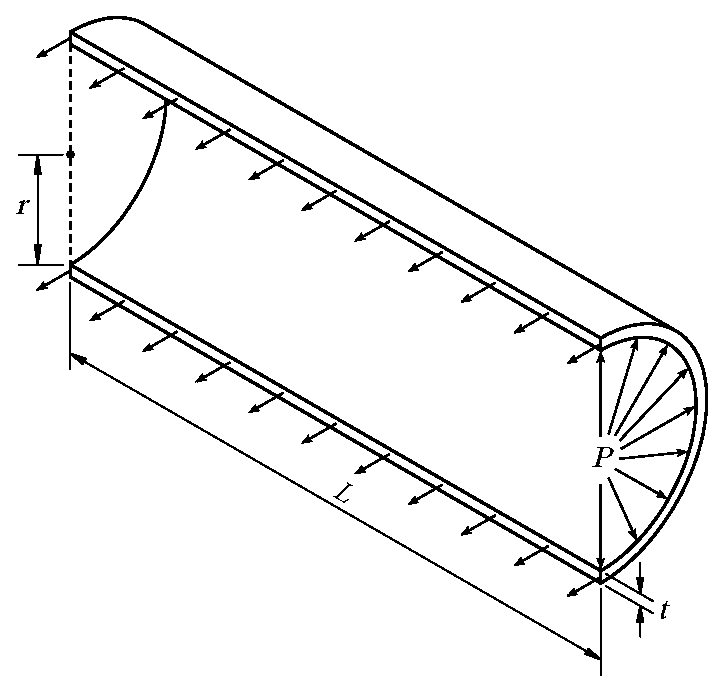
\includegraphics[width=3in]{PVessel}
\caption{Free-body diagram of the pressures acting on the pressure vessel internally.}
\label{fig:PVessel}
\end{figure}

The force balance for this diagram is \eqref{eq:vesselForce},
\begin{equation}
\label{eq:vesselForce}
(2rL)P=(2Lt)\sigma_H
\end{equation}
as pressure $P$ acts on the can inner surface area, $2rL$, and is resisted by the circumferential stress $\sigma_H$ acting on wall area $2Lt$.
The expression \eqref{eq:vesselForce} can be solved for the hoop stress $\sigma_H$ as \eqref{eq:hoopStress}.
\begin{equation}
\label{eq:hoopStress}
\sigma_H=\frac{Pr}{t}
\end{equation}

This hoop stress is related to its orthogonal longitudinal stress $\sigma_L$ with relationship \eqref{eq:longStress}, known from thin-walled pressure vessel theory \cite{b1}.
\begin{equation}
\label{eq:longStress}
\sigma_L=\frac{1}{2}\sigma_H
\end{equation}

These hoop and longitudinal stresses are assumed to be the principal stresses $\sigma_1$ and $\sigma_2$.
Thus the relationships from \eqref{eq:hoopStress} and \eqref{eq:sigmas} can be rearranged to yield a functional relationship between principal strain and internal pressure \eqref{eq:princStrainFin} \cite{b1}.
\begin{equation}
\label{eq:princStrainFin}
\varepsilon_1=\frac{Pr}{2Et}(2-\nu)
\end{equation}

\section{Procedure}

\subsection{Instrumenting the Soda Can}

The can must first be outfitted with the strain  gauge rosette.
First, the decorative wrapping on the beverage can is scrubbed off with methanol so that this wrapping does not affect the strain of the aluminum.
Once the surface is properly cleaned, painter's tape is used to create an approximately 90$^\circ$ L-shaped guideline towards the outer left and bottom edges of the cleaned surface for strain gauge placement.

To place the strain gauge rosette, clear packing tape is placed over the top of the rosette, opposite the side that will contact the surface of the can.
The tacky side of the taped strain rosette is then gently laid onto the can surface, such that the 0$^\circ$ and 90$^\circ$ strain gauges are aligned with the taped guidelines.
When the placement of the strain rosette is properly aligned, part of the taped side is lifted, and glue is applied to the can.
The strain gauge rosette is replaced over top of the glue and allowed to cure.

\subsection{Wheatstone Bridge}

Each strain gauge works as a variable resistor in a Wheatstone bridge, whose voltage difference is recorded for the strain.
Three Wheatstone bridge configurations are wired onto a simple breadboard.
Each bridge also makes use of a pre-amplifier, as the voltages passing through the circuit are expected to be very small.
An excitation voltage of 3.3 V is wired so as to pass across each bridge from an external power supply.
This excitation voltage $V_s$ and the voltage difference $V_{amp}$ for each of the three bridges is recorded with a SADI DAQ device.

\subsection{Data Acquisition}

The SADI DAQ which records the voltage difference is fed into a LabVIEW virtual instrument.
The LabVIEW VI reads the $V_{amp}$ for each bridge as $V_{amp_{x}}$ for the 0$^\circ$ gauge, $V_{amp_{t}}$  for the 45$^\circ$ gauge, and $V_{amp_{y}}$ for the 90$^\circ$ gauge.
These are observed with a $\pm$5.12 V gain window.

\subsection{Ideal Gas Law Pressure Determination Method}

A secondary method is also used based upon the ideal gas law.
For this method, the temperature of the room is measured and the can is allowed to reach thermodynamic equilibrium with the room.
The unopened, instrumented can is weighed on the lab scale, and its initial weight is recorded.
After the can is opened, the instrumented can is weighed again to record its final weight.
Next, a bottle filled with an arbitrary amount of water is weighed on the lab scale.
Water is poured from the bottle into the open can until the headspace between the soda and the top of the can is filled.
The bottle is weighed again.

\section{Results}

\lipsum[9-10]

\section{Discussion}

\lipsum[11-20]

\begin{figure}[H]
\label{fig:VampTime}
\def\svgwidth{3in}
\incfig{VampTime}
\caption{Graph thing}
\end{figure}

\begin{figure}[H]
\centering
\label{fig:2dSquare}
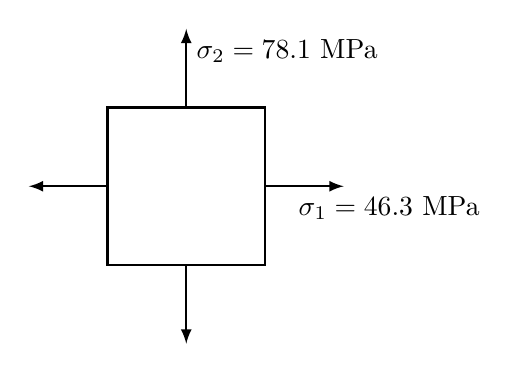
\begin{tikzpicture}
%square
\draw[thick] (-1,1) -- (1,1) -- (1,-1) -- (-1,-1) -- cycle;

%arrows
\draw[thick,-latex] (0,1) -- (0,2) node[below right] {$\sigma_2=78.1$ MPa};
\draw[thick,-latex] (1,0) -- (2,0)  node[below=8pt,right=-2em] {$\sigma_1=46.3$ MPa};
\draw[thick,-latex] (0,-1) -- (0,-2);
\draw[thick,-latex] (-1,0) -- (-2,0);
\end{tikzpicture}
\caption{2D principal stress element for pressure vessel.}
\end{figure}

\begin{figure}[H]
\centering
\label{fig:Mohr}
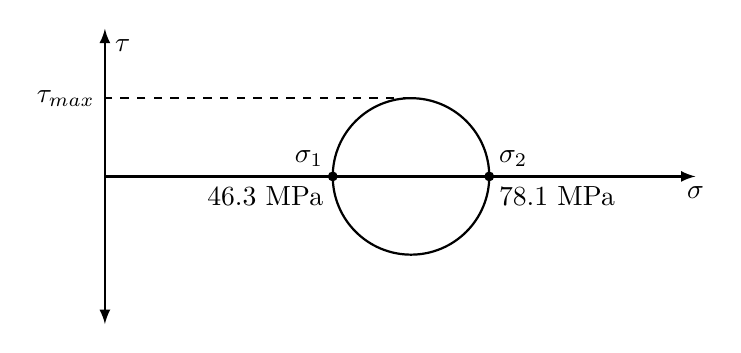
\begin{tikzpicture}[scale=0.625]
%axis
\draw[thick,latex-latex] (0,-3) -- (0,3) node[anchor=north west] {$\tau$};
\draw[thick,-latex] (0,0) -- (12,0) node[anchor=north] {$\sigma$};

%circle
\draw[thick] (6.22,0) circle (1.59);

%taumax
\draw[thick,dashed] (6.22,1.59) -- (0,1.59) node[left] {$\tau_{max}$};

%nodes
\filldraw[black] (4.63,0) circle (2.5pt);
\node[above left] at (4.63,0) {$\sigma_1$};
\node[below left] at (4.63,0) {46.3 MPa};
\filldraw[black] (7.81,0) circle (2.5pt);
\node[above right] at (7.81,0) {$\sigma_2$};
\node[below right] at (7.81,0) {78.1 MPa};
\end{tikzpicture}
\caption{Principal stresses plotted on Mohr’s circle diagram.}
\end{figure}

\section{Conclusion}

\lipsum[21]

\section*{Appendix A: Uncertainty Calculation}

The uncertainty of each variable is given by Table \ref{tab:Uncertainty}.
The uncertainties in $V_{amp_{x}}$, $V_{amp_{t}}$, $V_{amp_{y}}$, and $V_{s}$ were calculated by finding the standard deviation of a large sample set of these measurements and approximating a 95\% confidence interval.
The uncertainties in $d$ and $t$ were determined from the measuring device used, which was a micrometer.
The uncertainties in the weights of the can and the water were determined from the scale that was used and analyzing the sensitivity of the last digit.
The uncertainties in $E$, $\nu$, $R$, $M$, and $\rho$ were estimated to be $\pm$1\% of the given value due to variability associated with these material properties \cite{b8}.
\begin{table}[H]
\renewcommand\arraystretch{1.25}
\centering
\caption{Uncertainty in Each Variable}
\resizebox{3.5in}{!}{\begin{tabular}{ccc}
\hline \hline
Variable (Symbol) & Value & Uncertainty \\
\hline
Initial Amplified Voltage $x$ ($V_{amp_{xi}}$) & $-$0.1389 V & $\pm$0.00056 V \\
Initial Amplified Voltage $\theta$ ($V_{amp_{\theta i}}$) & 0.0673 V & $\pm$0.00039 V \\
Initial Amplified Voltage $y$ ($V_{amp_{yi}}$) & $-$0.1064 V & $\pm$0.00052 V \\
Final Amplified Voltage $x$ ($V_{amp_{xf}}$) & $-$0.237 V & $\pm$0.0011 V \\
Final Amplified Voltage $\theta$ ($V_{amp_{\theta f}}$) & $-$0.0253 V & $\pm$0.00027 V \\
Final Amplified Voltage $y$ ($V_{amp_{yf}}$) & $-$0.1398 V & $\pm$0.00055 V \\
Excitation Voltage ($V_s$) & 3.348 V &  $\pm$0.0015 V \\
Can Diameter ($d$) & 65.9 mm & $\pm$0.896 mm \\
Can Thickness ($t$) & 0.09 mm & $\pm$0.016 mm \\
Modulus of Elasticity ($E$) \cite{b3} & 69 GPa & $\pm$0.69 GPa \\
Poisson's Ratio ($\nu$) \cite{b3} & 0.35 & $\pm$0.0035 \\
%Shear Modulus ($G$) \cite{b3} & 25 GPa & $\pm$0.25 GPa \\
Gauge Factor ($G_f$) & 2.09 & $\pm$0.01045 \\
Gain ($A$) & 64 & $\pm$0.64 \\
Initial Can Weight ($W_{ci}$) & 406.8 g & $\pm$0.1 g \\
Final Can Weight ($W_{cf}$) & 406.2 g & $\pm$0.1 g \\
Initial Water Weight ($W_{wi}$) & 152.0 g & $\pm$0.1 g \\
Final Water Weight ($W_{wf}$) & 141.4 g & $\pm$0.1 g \\
Temperature ($T$) & 22.8$^\circ$C & $\pm$0.28$^\circ$C \\
Gas Constant ($R$) \cite{b6} & 8.31 \unit{\joule\per\kelvin\per\mole} & $\pm$0.083 \unit{\joule\per\kelvin\per\mole} \\
CO\textsubscript{2} Molar Mass ($M$) \cite{b4} & 44 \unit{\gram\per\mole} & $\pm$0.44 \unit{\gram\per\mole} \\
Density of Water ($\rho$) \cite{b7} & 0.998 \unit{\gram\per\centi\meter\cubed} & $\pm$0.00998 \unit{\gram\per\centi\meter\cubed} \\
\hline \hline
\end{tabular}}
\label{tab:Uncertainty}
\end{table}

\subsection*{Uncertainty in $\Delta V_{amp}$}

The change in $V_{amp}$ for each strain gauge can be calculated using \eqref{eq:deltaVamp}, where $V_{amp_{xi}}$, $V_{amp_{\theta i}}$, and $V_{amp_{yi}}$ are the initial voltages and $V_{amp_{xf}}$, $V_{amp_{\theta f}}$, and $V_{amp_{yf}}$ are the final voltages.
\begin{subequations}
\label{eq:deltaVamp}
\begin{align}
\Delta V_{amp_{x}}&=V_{amp_{xf}}-V_{amp_{xi}} \\
\Delta V_{amp_{\theta}}&=V_{amp_{\theta f}}-V_{amp_{\theta i}} \\
\Delta V_{amp_{y}}&=V_{amp_{yf}}-V_{amp_{yi}}
\end{align}
\end{subequations}
The uncertainty in each $\Delta V_{amp}$ can be calculated using the root sum square (RSS) method and \eqref{eq:deltaVamp}, where $U$ is the uncertainty.
\begin{equation}
\label{eq:UDeltaVamp}
\resizebox{227pt}{!}{$U_{\Delta V_{amp}}=\left[U_{V_{amp_{i}}}^2 \left(\frac{\partial (\Delta V_{amp})}{\partial V_{amp_{i}}}\right)^2 + U_{V_{amp_{f}}}^2 \left(\frac{\partial (\Delta V_{amp})}{\partial V_{amp_{f}}}\right)^2 \right]^{\frac{1}{2}}$}
\end{equation}
For $V_{amp_{x}}$, using the values given in Table \ref{tab:Uncertainty} give an uncertainty in $\Delta V_{amp_{x}}$ of $\pm$0.27 V.

\subsection*{Uncertainty in Strain}

Strain is given by \eqref{eq:strain}.
The uncertainty in strain can be calculated by using \eqref{eq:UStrain}.
\begin{equation}
\label{eq:UStrain}
\resizebox{227pt}{!}{$U_{\varepsilon}=\left[U_{\Delta V_{amp}}^2 \left(\frac{\partial \varepsilon}{\partial (\Delta V_{amp})}\right)^2 + U_{A}^2 \left(\frac{\partial \varepsilon}{\partial A}\right)^2 + U_{V_s}^2 \left(\frac{\partial \varepsilon}{\partial V_s}\right)^2 + U_{G_f}^2 \left(\frac{\partial \varepsilon}{\partial G_f}\right)^2 \right]^{\frac{1}{2}}$}
\end{equation}
For $V_{amp_{x}}$, using Table \todo\ and the values given in Table \ref{tab:Uncertainty} give an uncertainty in strain $\varepsilon_x$ of $\pm$0.0025 mm/mm.

\subsection*{Uncertainty in Shear Strain}

Shear strain is given by (\todo).
The uncertainty in shear strain can be calculated by using \eqref{eq:UShearStrain}.
\begin{equation}
\label{eq:UShearStrain}
U_{\gamma_{xy}}=\left[U_{\varepsilon_x}^2 \left(\frac{\partial \gamma_{xy}}{\partial \varepsilon_x}\right)^2 + U_{\varepsilon_t}^2 \left(\frac{\partial \gamma_{xy}}{\partial \varepsilon_t}\right)^2 + U_{\varepsilon_y}^2 \left(\frac{\partial \gamma_{xy}}{\partial \varepsilon_y}\right)^2 \right]^{\frac{1}{2}}
\end{equation}
Using Table \todo, the uncertainty in shear strain is $\pm$0.0015 mm/mm.

\subsection*{Uncertainty in Principle Strain}

Principle strain is given by \eqref{eq:princStrain}.
The uncertainty in principle strain can be calculated by using \eqref{eq:UPrincStrain}.
\begin{equation}
\label{eq:UPrincStrain}
\resizebox{227pt}{!}{$U_{\varepsilon_{1,2}}=\left[U_{\varepsilon_x}^2 \left(\frac{\partial \varepsilon_{1,2}}{\partial \varepsilon_x}\right)^2 + U_{\varepsilon_y}^2 \left(\frac{\partial \varepsilon_{1,2}}{\partial \varepsilon_y}\right)^2 + U_{\gamma_{xy}}^2 \left(\frac{\partial \varepsilon_{1,2}}{\partial \gamma_{xy}}\right)^2 \right]^{\frac{1}{2}}$}
\end{equation}
For $\varepsilon_1$, using Table \todo\ gives an uncertainty in principle strain $\varepsilon_1$ of $\pm$0.0024 mm/mm.

\subsection*{Uncertainty in Principle Stress}

Principle stress is given by \eqref{eq:sigmas}.
The uncertainty in principle stress can be calculated by using \eqref{eq:UPrincStress}.
\begin{equation}
\label{eq:UPrincStress}
\resizebox{227pt}{!}{$U_{\sigma_{1,2}}=\left[U_{E}^2 \left(\frac{\partial \sigma_{1,2}}{\partial E}\right)^2 + U_{\nu}^2 \left(\frac{\partial \sigma_{1,2}}{\partial \nu}\right)^2 + U_{\varepsilon_1}^2 \left(\frac{\partial \sigma_{1,2}}{\partial \varepsilon_1}\right)^2 + U_{\varepsilon_2}^2 \left(\frac{\partial \sigma_{1,2}}{\partial \varepsilon_2}\right)^2 \right]^{\frac{1}{2}}$}
\end{equation}
For $\sigma_1$, using Table \todo\ and the values given in Table \ref{tab:Uncertainty} gives an uncertainty in principle stress $\sigma_1$ of $\pm$0.19 GPa.

\subsection*{Uncertainty in Pressure from Strain}

Pressure from strain is given by (\todo).
The uncertainty in pressure can be calculated by using \eqref{eq:UPressStrain}.
\begin{equation}
\label{eq:UPressStrain}
U_{P}=\left[U_{\sigma_{1,2}}^2 \left(\frac{\partial P}{\partial \sigma_{1,2}}\right)^2 + U_{t}^2 \left(\frac{\partial P}{\partial t}\right)^2 + U_{d}^2 \left(\frac{\partial P}{\partial d}\right)^2 \right]^{\frac{1}{2}}
\end{equation}
Using Table \todo\ and the values given in Table \ref{tab:Uncertainty} gives an uncertainty in pressure from strain of $\pm$43.4 kPa.

\subsection*{Uncertainty in Amount of Substance}

The amount of substance $n$ is given by (\todo).
The uncertainty in the amount of substance can be calculated by using \eqref{eq:Uamt}.
\begin{equation}
\label{eq:Uamt}
\resizebox{227pt}{!}{$U_{n}=\left[U_{W_{ci}}^2 \left(\frac{\partial n}{\partial W_{ci}}\right)^2 + U_{W_{cf}}^2 \left(\frac{\partial n}{\partial W_{cf}}\right)^2 + U_{M}^2 \left(\frac{\partial n}{\partial M}\right)^2 \right]^{\frac{1}{2}}$}
\end{equation}
Using Table \todo\ and the values given in Table \ref{tab:Uncertainty} gives an uncertainty in the amount of substance of $\pm$43.4 mol.

\subsection*{Uncertainty in Volume}

Volume is given by (\todo).
The uncertainty in volume can be calculated by using \eqref{eq:Uvol}.
\begin{equation}
\label{eq:Uvol}
\resizebox{227pt}{!}{$U_{V}=\left[U_{W_{wi}}^2 \left(\frac{\partial V}{\partial W_{wi}}\right)^2 + U_{W_{wf}}^2 \left(\frac{\partial V}{\partial W_{wf}}\right)^2 + U_{\rho}^2 \left(\frac{\partial V}{\partial \rho}\right)^2 \right]^{\frac{1}{2}}$}
\end{equation}
Using Table \todo\ and the values given in Table \ref{tab:Uncertainty} gives an uncertainty in volume of $\pm$0.108 \unit{\centi\meter\cubed}.

\subsection*{Uncertainty in Pressure from Ideal Gas Law}

Pressure from the ideal gas law is given by (\todo).
The uncertainty in pressure can be calculated by using \eqref{eq:UPressIGL}.
\begin{equation}
\label{eq:UPressIGL}
\resizebox{227pt}{!}{$U_{P_{IGL}}=\left[U_{n}^2 \left(\frac{\partial P_{IGL}}{\partial n}\right)^2 + U_{R}^2 \left(\frac{\partial P_{IGL}}{\partial R}\right)^2 + U_{T}^2 \left(\frac{\partial P_{IGL}}{\partial T}\right)^2 + U_{V}^2 \left(\frac{\partial P_{IGL}}{\partial V}\right)^2 \right]^{\frac{1}{2}}$}
\end{equation}
Using Table \todo\, the values given in Table \ref{tab:Uncertainty}, and the uncertainties calculated in the previous sections gives an uncertainty in pressure from the ideal gas law of $\pm$57.2 kPa.

%\hfill\break
%\noindent
%This lab report was produced using \LaTeX.

\begin{thebibliography}{00}
\bibitem{b1} G. Subhash and S. Ridgeway, ``Thin-walled Pressure Vessels," in \textit{Mechanics of Materials Laboratory Course}. San Rafael, CA: Morgan \& Claypool, 2018, ch. 3, pp. 113--132.
\bibitem{b5} S. Ridgeway. (2022). Lab 3 Discussion, Final Project Track 1 [PowerPoint slides]. Available: \url{https://ufl.instructure.com/courses/447927/files/67779901}
\bibitem{b2} D. R. Askeland, F. Haddleton, P. Green, and H. Robertson, ``Nonferrous Alloys," in \textit{The Science and Engineering of Materials}, 3rd ed. Berlin, Germany: Springer, 1996, ch. 13, pp. 401--436.
\bibitem{b3} J. W. Bray, ``Aluminum Mill and Engineered Wrought Products," in \textit{Properties and Selection: Nonferrous Alloys and Special-Purpose Materials} (ASM Handbook, Vol. 2). Russell Township, OH: ASM International, 1990.
\bibitem{b4} Engineering ToolBox. (2018). \textit{Carbon Dioxide - Thermophysical Properties}. [Online] Available: \url{https://www.engineeringtoolbox.com/CO2-carbon-dioxide-properties-d_2017.html}
\bibitem{b6} Engineering ToolBox. (2004). \textit{Universal and Individual Gas Constants}. [Online] Available: \url{https://www.engineeringtoolbox.com/individual-universal-gas-constant-d_588.html}
\bibitem{b7} Engineering ToolBox. (2003). \textit{Water - Density, Specific Weight and Thermal Expansion Coefficients}. [Online] Available: \url{https://www.engineeringtoolbox.com/water-density-specific-weight-d_595.html}
\bibitem{b8} S. Ridgeway. (2022). Lab 2 Report, Uncertainty [PowerPoint slides]. Available: \url{https://ufl.instructure.com/courses/447927/files/66505329}
\bibitem{b9} H. de Grys, ``Determining the pressure inside an unopened carbonated beverage," Journal of Chemical Education, vol. 84, no. 7, p. 1117, 2007.
\end{thebibliography}

\end{document}